\subsubsection*{10.a}
On va afficher les id(column\_id) , nom(column\_name) , type de donnes(data\_type) , nullabilite(nullable) , valeur par defaut(data\_default)
des attributs de la table SUBSCRIBE en utilisant la table USER\_TAB\_COLUMNS et bien sure le where pour just selectionner la table SUBSCRIBE
where table\_name='SUBSCRIBE'

\lstinputlisting[style=sqlstyle]{SQL/Partie5/att.sql}

\begin{center}
    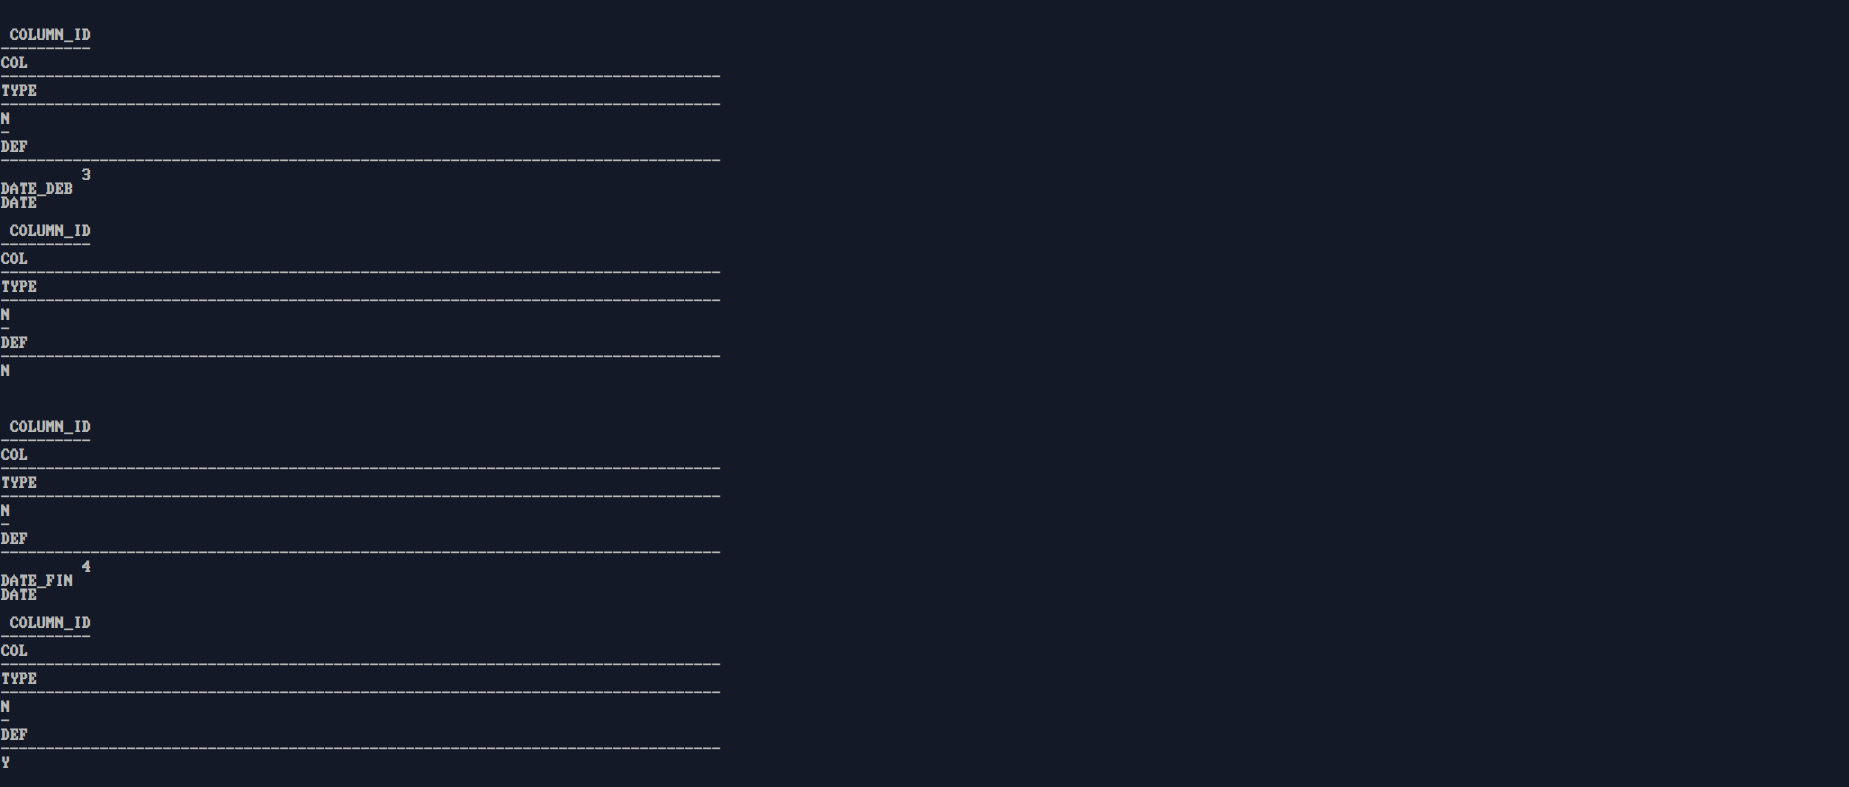
\includegraphics[width=\textwidth]{ScreenShot/Partie5/att.png}
\end{center}

\subsubsection*{10.b}
Pour obtenir le nom de la contrainte cle primaire et les nom de ces attributs  on va faire
une jointure entre USER\_CONSTRIANTS et USER\_CONS\_COLUMNS , la premiere table va nous aider
a filterer les contraintes pour just avoir des contraintes de type cle primaire \\t1.constraint\_type = 'P' 
de la table SUBSCRIBE t1.table\_name='SUBSCRIBE' puis on utilise la deuxieme table pour afficher les noms des attributs de la cle primaire
t2.column\_name avec la jointure t1.constraint\_name=t2.constraint\_name

\lstinputlisting[style=sqlstyle]{SQL/Partie5/pk.sql}

\begin{center}
    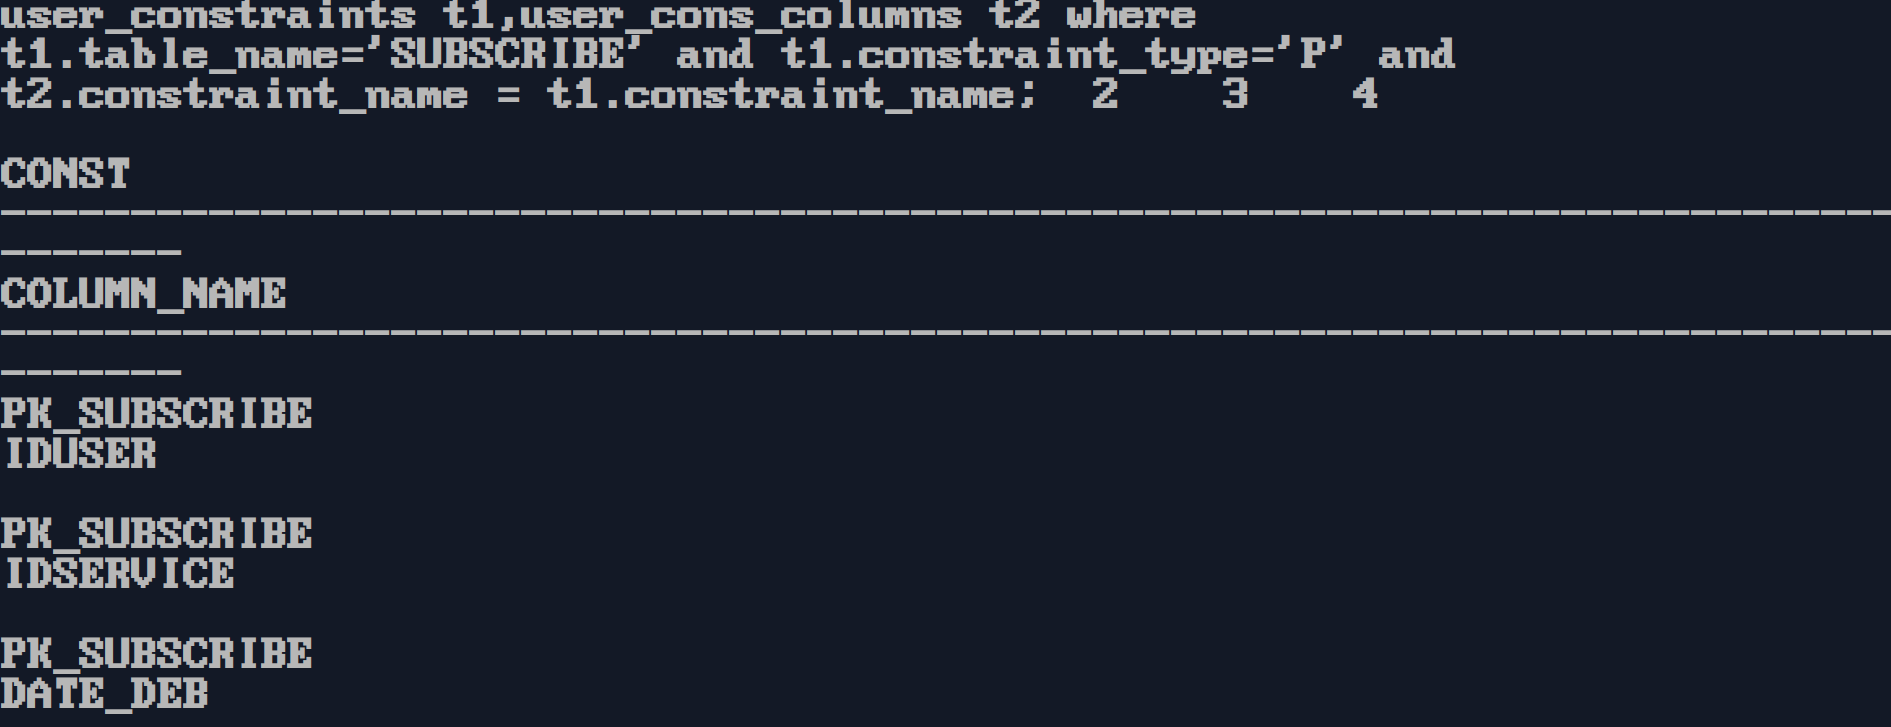
\includegraphics[width=\textwidth]{ScreenShot/Partie5/pk.png}
\end{center}

\subsubsection*{10.c}
Pour afficher les nom des contraintes cle etrangers et le nom de l'attribut , table reference , colonne reference on doit utiliser des imbriquation de select 
toujours avec les deux table USER\_CONSTRIANTS et USER\_CONS\_COLUMNS , le outer select fait une jointure entre les tables et affiche le nom de la contrainte
et son attribut en filtron le type pour foreign key t1.constraint\_type = 'R' de la table SUBSCRIBE t1.table\_name='SUBSCRIBE' , pour afficher la table reference
on va selectioner le nom de la table de la contrainte cle primaire reference par la table SUBSCRIBE t1.r\_constraint\_name=t11.constraint\_name depuis la table
USER\_CONSTRAINTS, pour affiche les colonnes reference
en selectionne les nom des colonnes de la contrainte cle primaire reference par la table SUBSCRIBE de puis la table USER\_CONS\_COLUMNS t1.r\_constraint\_name=t22.constraint\_name 

\lstinputlisting[style=sqlstyle]{SQL/Partie5/fr1.sql}

\begin{center}
    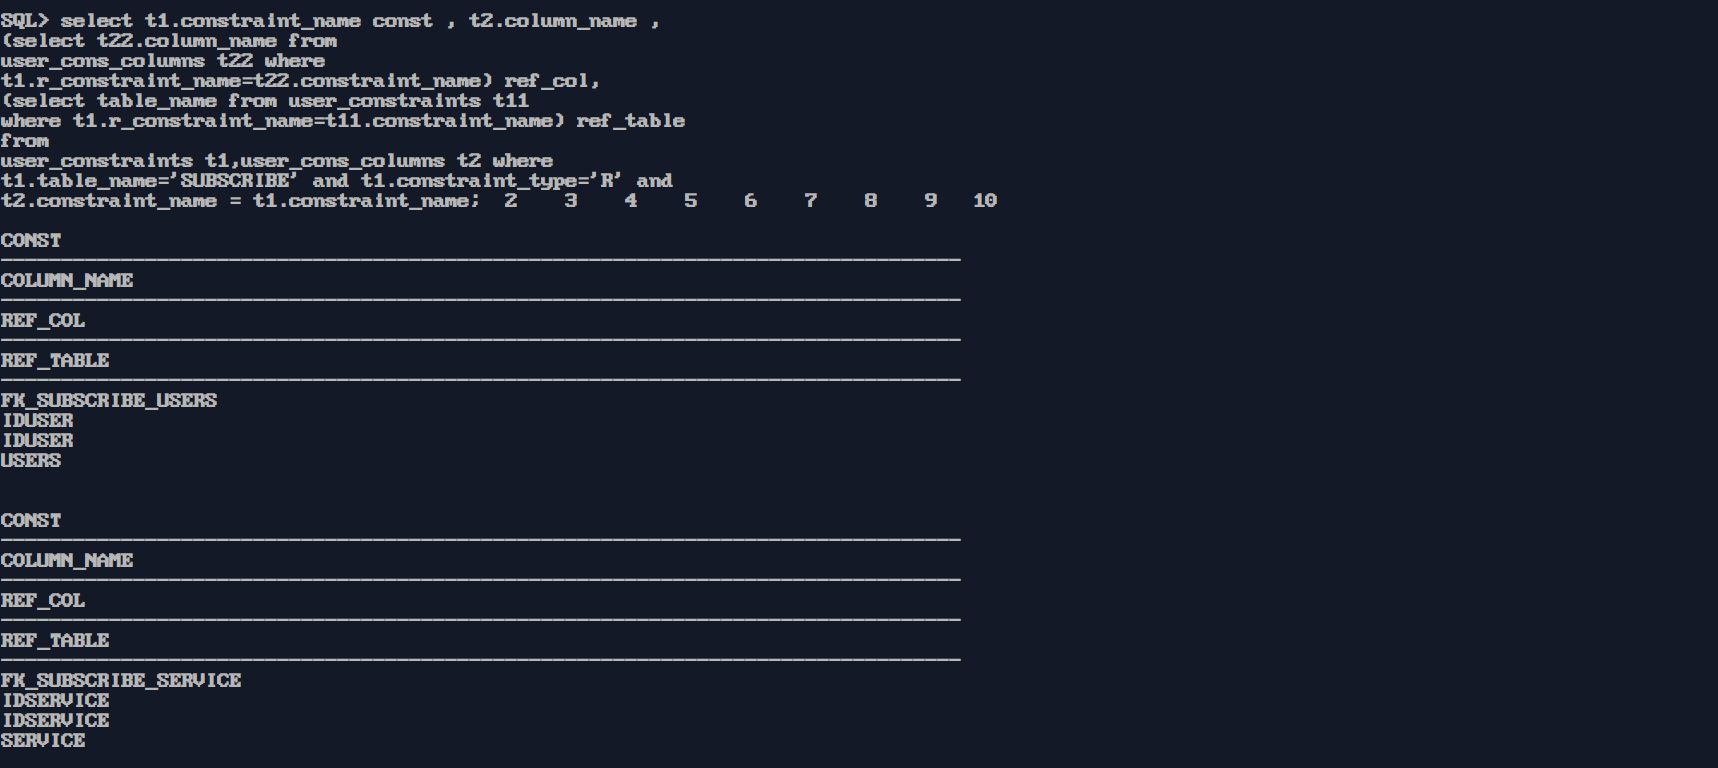
\includegraphics[width=\textwidth]{ScreenShot/Partie5/fr1.png}
\end{center}

\subsubsection*{10.d}
Pour obtenir les nom des contraintes uniques et les nom des attributs associes on va faire
une jointure entre USER\_CONSTRIANTS et USER\_CONS\_COLUMNS , la premiere table va nous aider
a filterer les contraintes pour just avoir des contraintes de type unique \\t1.constraint\_type = 'U' 
de la table SUBSCRIBE t1.table\_name='SUBSCRIBE' puis on utilise la deuxieme table pour afficher le nom de l'attribut unique
t2.column\_name avec la jointure t1.constraint\_name=t2.constraint\_name

\lstinputlisting[style=sqlstyle]{SQL/Partie5/uni.sql}

\begin{center}
    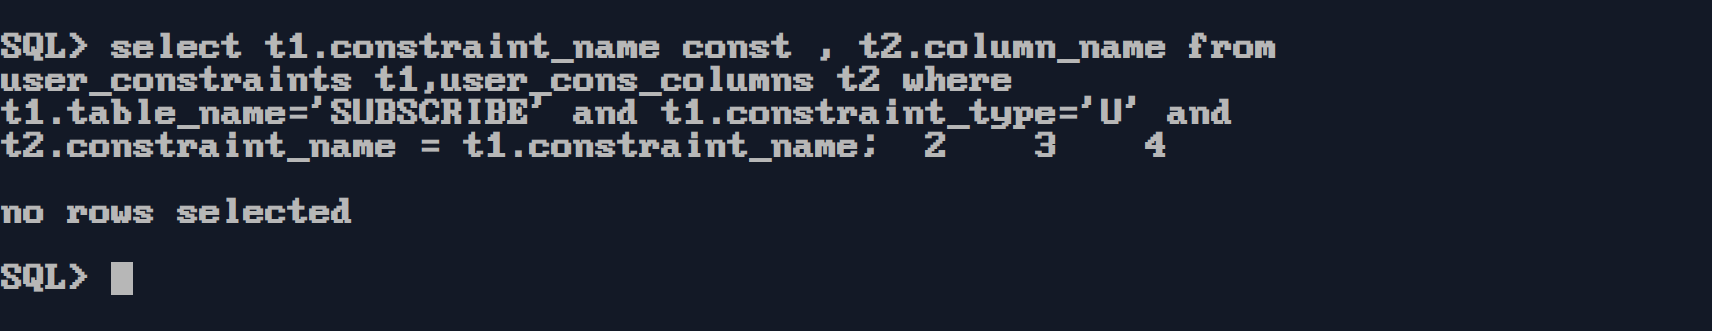
\includegraphics[width=\textwidth]{ScreenShot/Partie5/uni.png}
\end{center}

\subsubsection*{10.e}
On va obtenir les nom des contraints check + leur condition avec la table
USER\_CONSTRAINTS , on selectionnant l'attribut constraint\_name(nom de la contraint) ,
search\_condition(condition du check) et pour avoir que les contraintes de la table subscribe de type check
on utilise le where clause table\_name='SUBSCRIBE' and constraint\_type='C'(type check)

\lstinputlisting[style=sqlstyle]{SQL/Partie5/chk.sql}

\begin{center}
    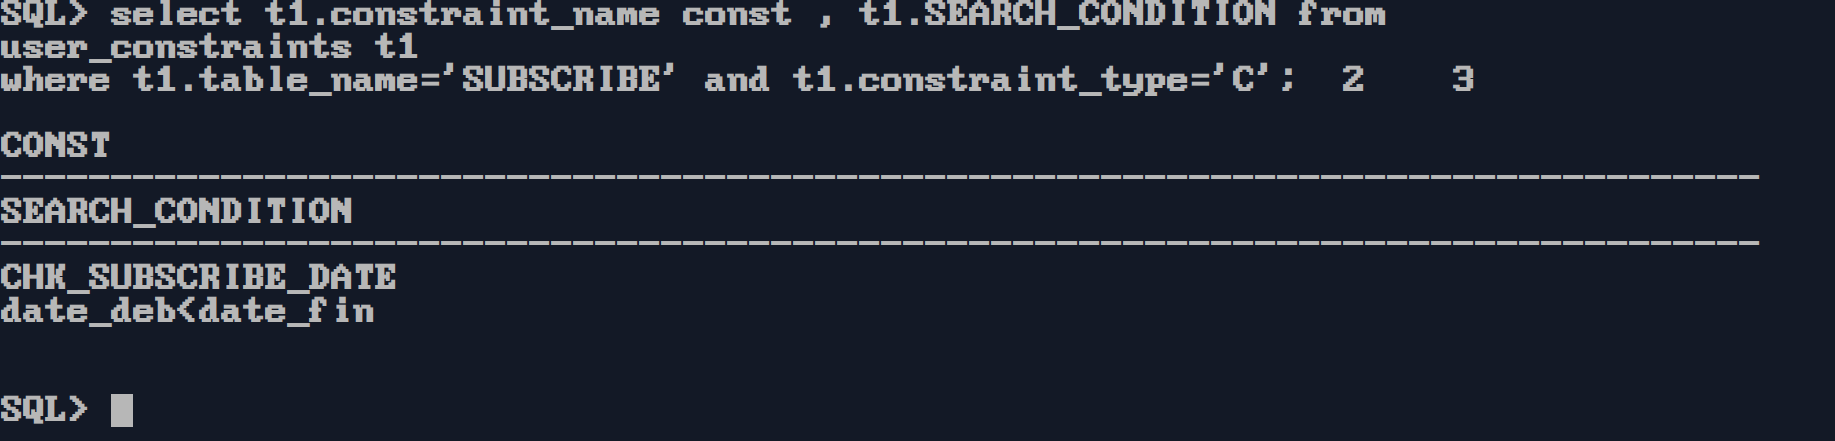
\includegraphics[width=\textwidth]{ScreenShot/Partie5/chk.png}
\end{center}





